% !TeX root = ../main.tex
% Add the above to each chapter to make compiling the PDF easier in some editors.

\chapter{Introduction}\label{chapter:introduction}

\textbf{Locking mechanism is important.}
In modern computing environments, the efficiency of locking mechanisms play a crucial role in the performance of various systems, including databases~\parencite{lomet1993key, graefe2007hierarchical}, file systems~\parencite{lee2021concurrent, gao2023citron, lee2019write}, and operating systems~\parencite{readerWriterLocks2017, mmapSem2017}. As these systems grow in scale and complexity, the demand for more sophisticated and efficient locking mechanisms becomes crucial. One of the fundamental challenges in this context is managing concurrent access to shared resources. Traditional locking techniques, such as single-lock mechanisms, often lead to significant performance bottlenecks, particularly in high-concurrency scenarios.

\textbf{Range locks boot performance through resource segmentation.} 
Range lock~\parencite{gao2023citron, kogan2020scalable} provide a more refined approach to this issue by partitioning a shared resource into multiple arbitrary-sized segments. Each of these segments can be exclusively acquired by different processes. This strategy effectively addresses the drawbacks and bottlenecks associated with single-lock methods, significantly improving the performance.

\textbf{DBMS needs range locks.}
As database sizes increase exponentially, locking the entire database becomes impractical. This approach will prevent concurrent transactions from progressing, resulting in poor throughput and high latency. The previous key-range locking in DBMS is complex and tightly coupled with lock-based concurrency control protocols~\parencite{graefe2007hierarchical, andy2022database}. 
Consequently, this technique is not applicable to general DBMS operations, such as variable-sized page allocation. Therefore, a new technique, such as range locks is desirable.

\textbf{Existing range lock need improvement.}
Previous implementations of range-locking mechanisms often need to improve their performance. These implementations often suffer from contention points due to the reliance on a single lock~\parencite{linuxRangeLockImpl2013, song2013parallelizing}. Additionally, some methods may be complex and tightly coupled with lock-based concurrency control protocols, which are not applicable for general DBMS operations~\parencite{graefe2007hierarchical, andy2022database}. These limitations underscore the need for more refined and scalable solutions that can better handle the demands of modern, large-scale systems.

\newpage

\textbf{New concurrent range-locking design.} In this research's scope, we propose a new concurrent range-locking design that leverages a probabilistic concurrent skip list~\parencite{herlihy2006provably, herlihy2020art}. Our range lock design also utilizes the per-node lock technique instead of an interval lock, thus addressing the previous range lock bottleneck problem and maintaining the lock's high level of performance.

\begin{figure}[h]
    \centering
    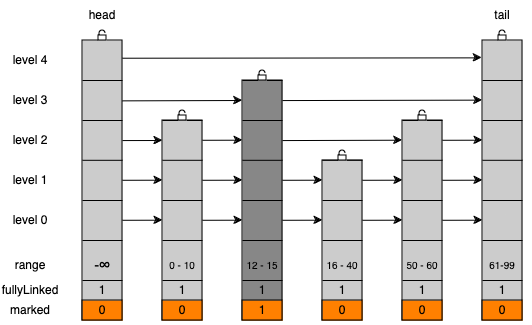
\includegraphics[width=0.8\textwidth]{./figures/concurrent_range_lock.png}
    \caption{Concurrent range lock}
    \label{fig:concurrent_range_lock}
\end{figure}

\textbf{Outline of the research.} The scope of this research includes developing and evaluating the proposed range-locking mechanism. We will evaluate focusing on performance under heavy concurrent accesses, ensuring the correctness of data access in overlapping ranges and concurrent operations. Additionally, we will compare the performance of the proposed solution with existing state-of-the-art approaches to provide a comprehensive assessment of its effectiveness.